% !TeX root = ../main.tex

\chapter{实验}
\label{cha:chapter05}

本章将使用前文设计并实现的动态社交网络图生成系统进行实验,检验动态社交网络图生成算法所产生结果的各项性质并展示生成过程的复杂度。

实验过程中使用的机器配置如下:

\begin{itemize}
  \item 处理器:2.7 GHz 双核Intel Core i5
  \item 内存:8 GB 1867 MHz DDR3
  \item 系统:macOS 10.15.3
\end{itemize}

\section{动态图特征分析}

本节将使用指定的配置信息进行动态图的生成,并且检测生成的图是否满足要求。

本节使用如下配置方式,检验入度分布与出度分布是否符合预期:

\begin{itemize}
  \item 总帧数为$10$
  \item 定义了标签为student的节点、标签为friend的边,节点总数为$2000$,不存在多重边
  \item 入度分布与出度分布为$\lambda=2$的Power-Law分布
  \item 社区按照$8:2$的比例进行划分,社区参数$\rho=0.5$
  \item 定义以下事件:
  \begin{itemize}
    \item 第3帧:节点重要度变化,影响$1\%$的节点
    \item 第5-7帧:突发事件导致$1\%$节点重要度上升
    \item 第6帧:社区更为明显,社区参数变化为$\rho=0.3$
    \item 第5帧:节点增加,新增$50$个节点
    \item 第9帧:节点删除,原有的$90$个节点被删除
  \end{itemize}
\end{itemize}

由于Power-Law分布的概率密度函数为指数形式,因此将入度分布与出度分布使用对数坐标轴呈现,度数范围为$[1, 100]$的结果如图\ref{fig:parallel1}与图\ref{fig:parallel2}所示。

\begin{figure}
\begin{minipage}{0.48\textwidth}
  \centering
  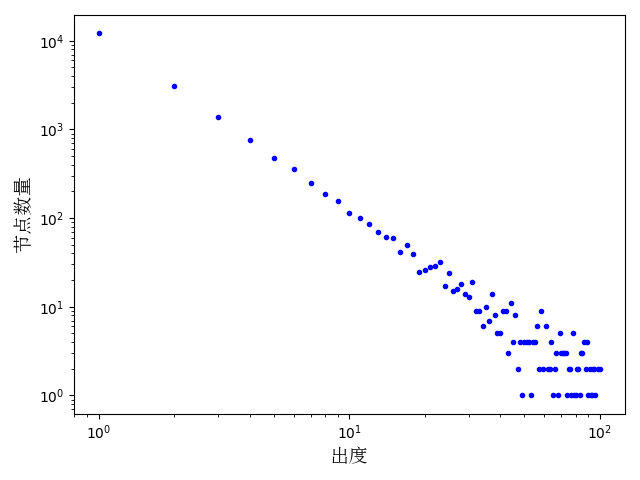
\includegraphics[scale=0.3]{out_degree_exp1.png}
  \caption{生成结果出度分布}
  \label{fig:parallel1}
\end{minipage}\hfill
\begin{minipage}{0.48\textwidth}
  \centering
  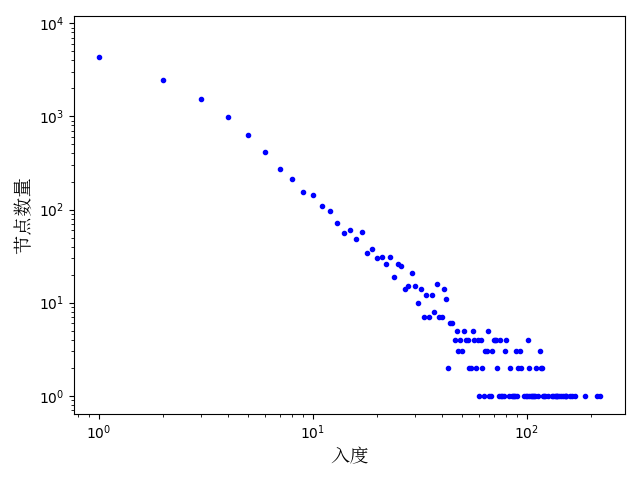
\includegraphics[scale=0.3]{in_degree_exp1.png}
  \caption{生成结果入度分布}
  \label{fig:parallel2}
\end{minipage}
\end{figure}

从图中可以看出,结果的出度分布范围与给定条件几乎完全吻合,从图上来看的确符合Power-Law分布。

总体来看,入度分布的确符合Power-Law分布。但入度分布与给定的条件并不完全相符,出现了许多度数超出配置时的度数范围($[1, 100]$)的节点。这是因为入度分布的信息只是提供目标节点选择概率的参考,由于入度分布于出度分布可能不相吻合,因此不会保证结果的入度分布完全符合给定的要求。

接下来检验单个节点的度数变化。为了避免度数极小的点对分析造成干扰,在此将度数范围设置为$[30, 100]$。

在此选择一些在事件中重要度发生变化的节点。如图\ref{fig:important_eg1}与图\ref{fig:important_eg2}所示,节点1514和节点326是节点重要度变化事件中受到影响的节点,其重要性分别在第3帧时得到提升与降低。

\begin{figure}[H]
  \centering
  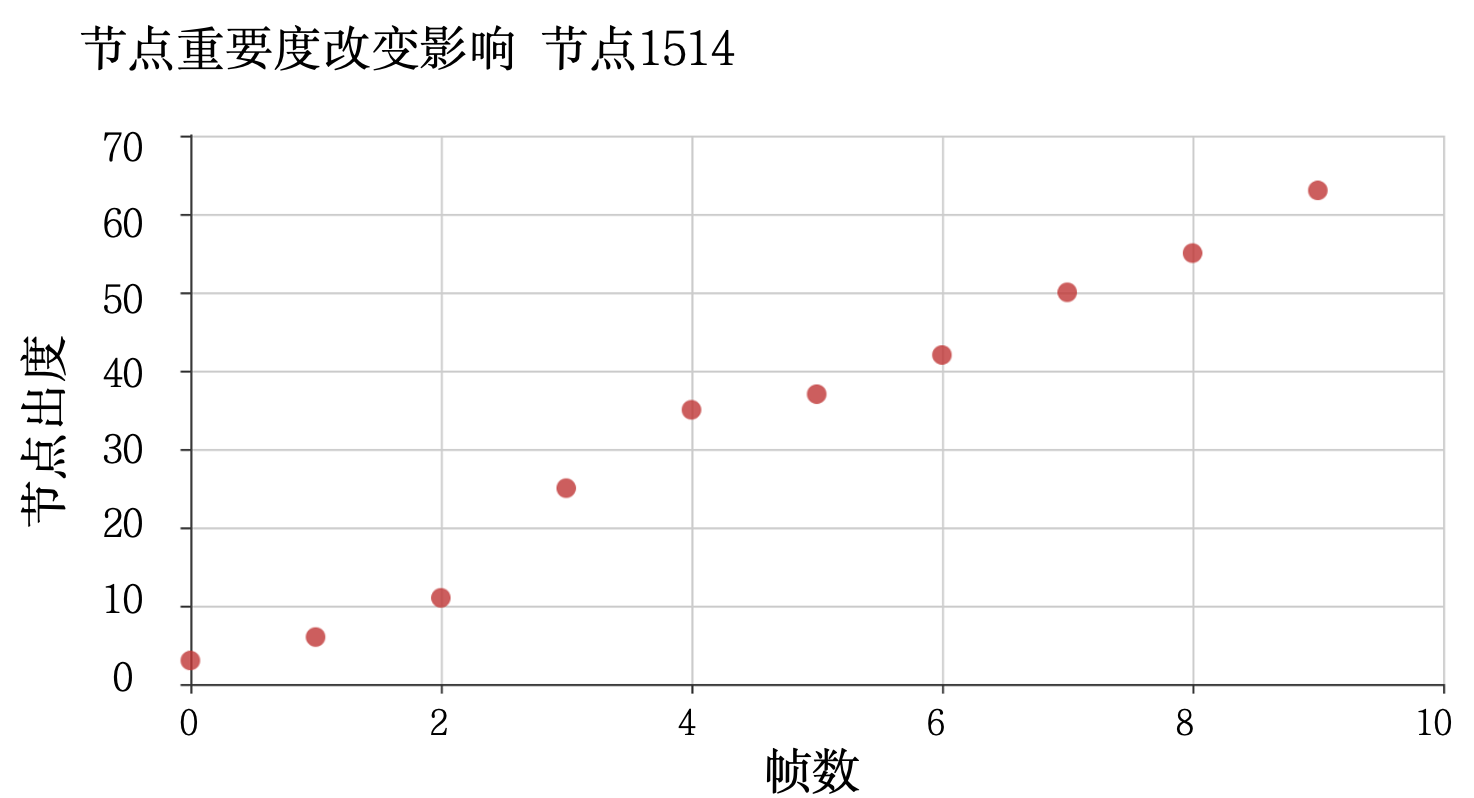
\includegraphics[scale=0.6]{important_eg1.png}
  \caption{节点重要度提升—以节点1514为例}
  \label{fig:important_eg1}
\end{figure}

\begin{figure}[H]
  \centering
  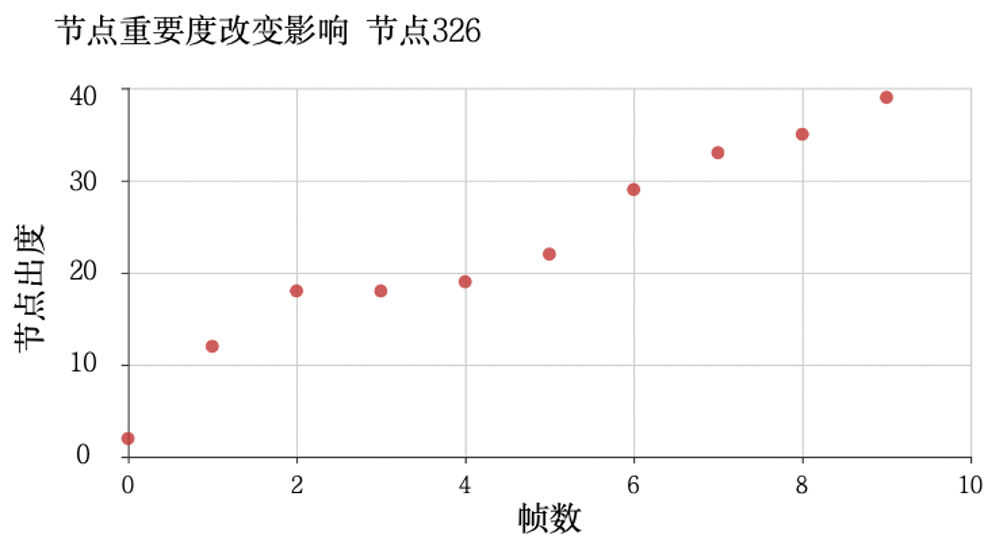
\includegraphics[scale=0.6]{important_eg2.png}
  \caption{节点重要度降低—以节点326为例}
  \label{fig:important_eg2}
\end{figure}

第5-7帧中的突发事件模拟代表着某些节点度数增长速度的临时加快。如图\ref{fig:sudden_event_eg}所示,节点1866在该事件中受到影响,第5-7帧中度数增长速度明显加快。

\begin{figure}[H]
  \centering
  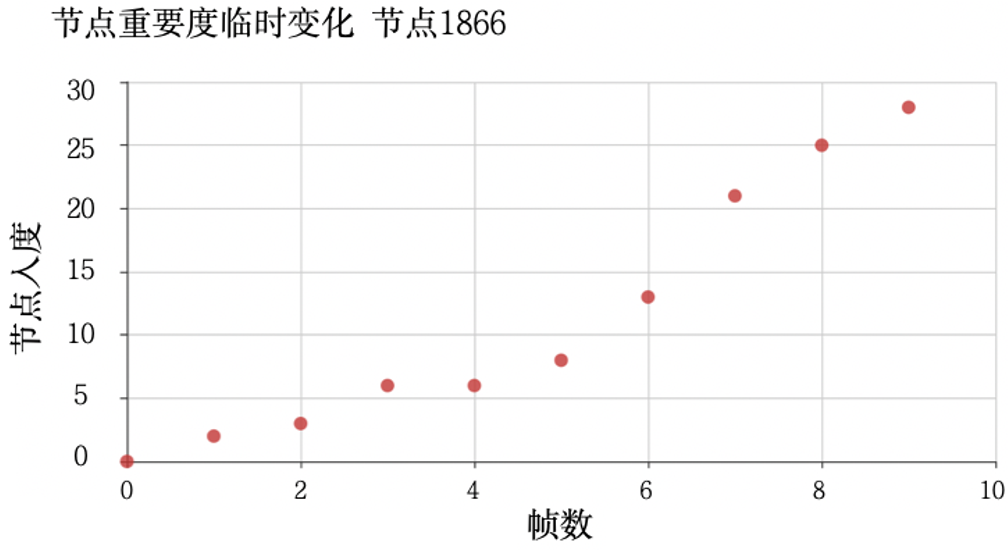
\includegraphics[scale=0.6]{sudden_event_eg.png}
  \caption{突发事件模拟—以节点1866为例}
  \label{fig:sudden_event_eg}
\end{figure}

接下来对生成结果的社区特征进行分析。此处将社区划分比例调整为$2:3:5$,并且将节点按照社区重排,结果如图\ref{fig:community_vis}所示。

\begin{figure}[H]
  \centering
  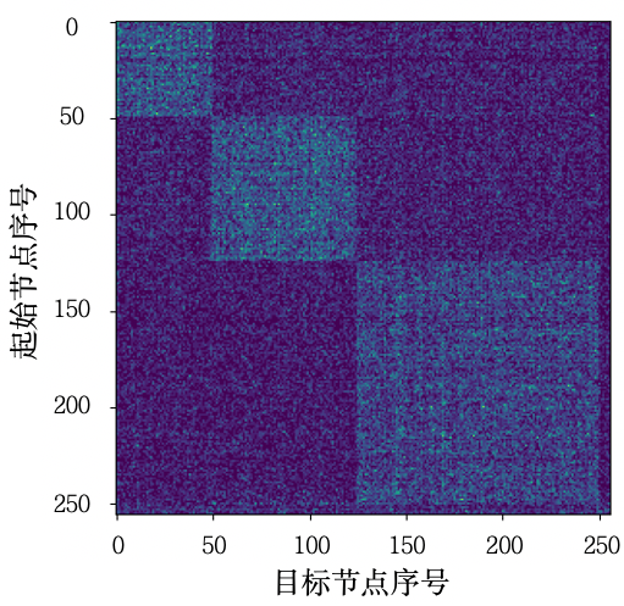
\includegraphics[scale=0.6]{community_vis.png}
  \caption{社区可视化}
  \label{fig:community_vis}
\end{figure}

我们可以清楚地看出其中的社区,这可以说明生成算法的结果符合给定的社区分布。

\section{性能分析}

此节旨在用不同的节点数、边数、帧数等配置信息进行生成,比较所用时间,用以验证生成算法的性能。

若无特殊说明,实验中共用的配置如下:

\begin{itemize}
  \item 定义了标签为student的节点、标签为friend的边,不存在多重边
  \item 出度分布采用$\lambda=2$、最大度数为100、最小度数可变的Power-Law分布
  \item 入度分布与出度分布定义方式相同
  \item 社区按照$8:2$的比例进行划分,社区参数$\rho=0.5$
  \item 不设置事件
  \item 使用ADJ格式进行存储
  \item 节点总数、分布的最小度数、边总数\footnote{边的实际数量由边生成过程中通过给定的出度分布确定}、帧数信息会分别在每个实验中说明
\end{itemize}

\subsection{所用时间随图规模的变化}

本节通过对节点数目、分布的最小度数这两项配置信息的修改,观察所用时间与图的整体规模的关系。实验中配置与结果如表\ref{tab:exp}所示。

\begin{table}[htb]
  \centering
  \caption[实验-所用时间随图规模的变化]{所用时间随图规模的变化}
  \label{tab:exp}
  \begin{minipage}[t]{0.8\textwidth}
    \begin{tabularx}{\linewidth}{lllll}
      \toprule[1.5pt]
      {\heiti 节点总数} & {\heiti 最小度数} & {\heiti 边总数} & {\heiti 帧数} & {\heiti 时间(s)} \\
      \midrule[1pt]
      100 & 3 & 867 & 10 & 0.114\\\hline
      100 & 30 & 5251 & 10 & 0.226\\\hline
      1000 & 3 & 9581 & 10 & 0.640\\\hline
      1000 & 30 & 51554 & 10 & 1.650\\\hline
      5000 & 3 & 47861 & 10 & 3.355\\\hline
      5000 & 30 & 254777 & 10 & 9.619\\\hline
      5000 & 90 & 499767 & 10 & 11.648\\\hline
      10000 & 3 & 93037 & 10 & 6.425\\\hline
      10000 & 30 & 515136 & 10 & 16.006\\\hline
      10000 & 90 & 947884 & 10 & 21.712\\\hline
      50000 & 3 & 476961 & 10 & 32.299\\\hline
      50000 & 30 & 2555196 & 10 & 81.717\\\hline
      50000 & 90 & 4736425 & 10 & 118.890\\\hline
      100000 & 3 & 953490 & 10 & 80.333\\\hline
      100000 & 30 & 5106549 & 10 & 190.093\\\hline
      100000 & 90 & 9475146 & 10 & 240.551\\
      \bottomrule[1.5pt]
    \end{tabularx}
  \end{minipage}
\end{table}

\begin{figure}[H]
  \centering
  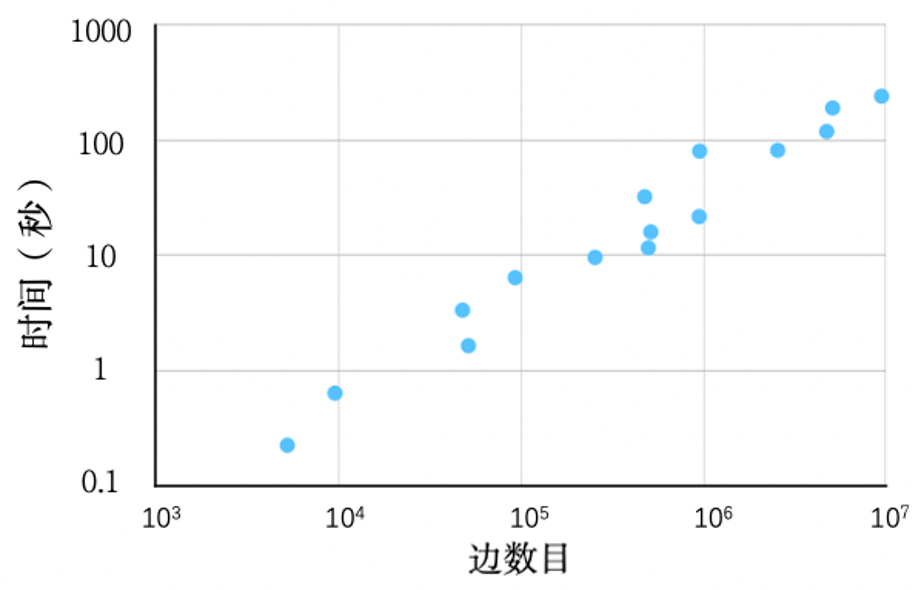
\includegraphics[scale=0.5]{edges_time.png}
  \caption{用时与边数目的关系}
  \label{fig:edges_time}
\end{figure}

将表中边数目与所用时间两项抽取出来,如图\ref{fig:edges_time}所示,可以看出总体时间的增长随边数目呈线性关系。

\subsection{所用时间随帧数的变化}

本节将节点数目、分布的最小度数固定,观察所用时间与总帧数的关系。

本实验的配置与结果如表\ref{tab:exp2}所示。

\begin{table}[htb]
  \centering
  \caption[实验-所用时间随帧数的变化]{所用时间随帧数的变化}
  \label{tab:exp2}
  \begin{minipage}[t]{0.8\textwidth}
    \begin{tabularx}{\linewidth}{lllll}
      \toprule[1.5pt]
      {\heiti 节点总数} & {\heiti 最小度数} & {\heiti 边总数} & {\heiti 帧数} & {\heiti 时间(s)} \\
      \midrule[1pt]
      10000 & 30 & 509966 & 1 & 3.096\\\hline
      10000 & 30 & 508252 & 3 & 7.663\\\hline
      10000 & 30 & 512508 & 9 & 14.937\\\hline
      10000 & 30 & 512150 & 27 & 37.837\\
      \bottomrule[1.5pt]
    \end{tabularx}
  \end{minipage}
\end{table}

\begin{figure}[H]
  \centering
  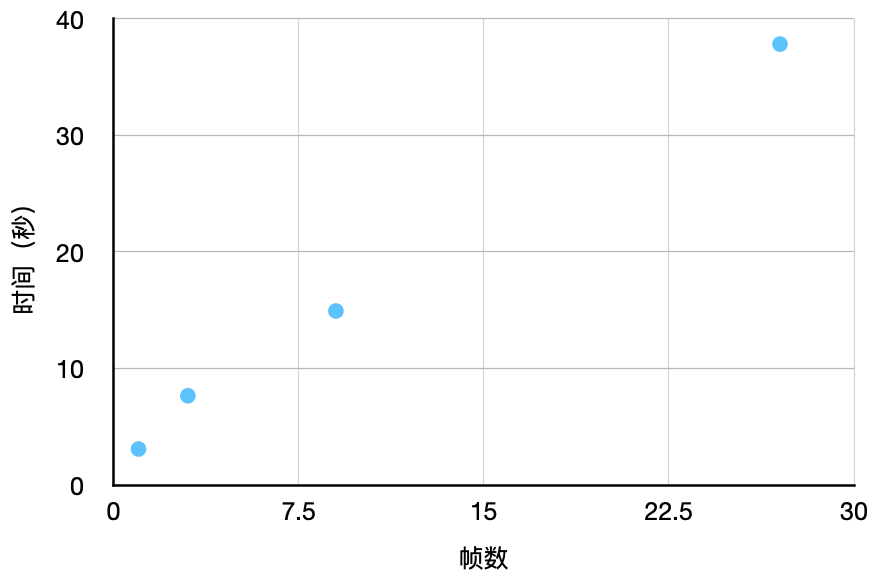
\includegraphics[scale=0.5]{time_stampnum.png}
  \caption{用时与帧数的关系}
  \label{fig:stamps_time}
\end{figure}

将表中帧数与所用时间两项抽取出来,如图\ref{fig:stamps_time}所示。从表\ref{tab:exp2}和图\ref{fig:stamps_time}中可以看出,所用时间与总帧数有着很大的关联,总耗时随着总帧数增加逐渐增长,速度略慢于线性关系。

更大的总帧数会导致每帧中的保存工作消耗更多的时间,并且总的循环次数增多会导致单次循环产生的边更少,生成效率更低。